\documentclass[10pt, twocolumn]{article}

%----------------------------------------------
%-----------------Packages---------------------
%----------------------------------------------

% Writing 
\usepackage[english]{babel}
\usepackage[utf8]{inputenc}
\usepackage[pdftex]{lscape}
\fontfamily{times}
\usepackage[affil-it]{authblk}
\usepackage{lettrine}

% Graphics
\usepackage{caption}
\usepackage{float}
\usepackage{subcaption}
\usepackage{graphicx}
\usepackage[outdir=./images/]{epstopdf}
\graphicspath{{images/}}

% Math
\usepackage{amsthm, amssymb, amsmath, mathtools}

% Biblio
\usepackage[numbers]{natbib}
\bibliographystyle{apalike}

%Others
\usepackage{url}
\usepackage[colorlinks=true,citecolor=blue,linkcolor=magenta]{hyperref}
\usepackage{ifthen}
\usepackage{multirow}

%----------------------------------------------
%---------------Math definitions---------------
%----------------------------------------------

\newcommand{\R}{\mathbb{R}}

%----------------------------------------------
%--------------Other definitions---------------
%----------------------------------------------

\newcommand{\com}[1]{\textcolor{red}{#1}}

%----------------------------------------------
%-----------------Title Page-------------------
%----------------------------------------------

\title{Machine Learning}

\author{Lucas Machado Moschen}
\affil{School of Applied Mathematics, \\ Fundação Getulio Vargas}

\date{\today}

%----------------------------------------------
%------------------Document--------------------
%----------------------------------------------


\begin{document}

\newcounter{num}
\setcounter{num}{0}

\twocolumn[
    \begin{@twocolumnfalse}

        \maketitle

        \begin{abstract}
            Air is an essential resource and its quality is important for the human being
and the environment. The ability to understand and predict air quality may
help to prevent events of poor quality and formulate environmental policies.
This work presents models for O$_3$, CO, and PM$_{10}$ for each monitoring
station in Rio de Janeiro. Machine learning methods, including linear
regression, support vector machine, and random forest produced promising
results for gases and AQI levels predictions. 

\vspace{6mm}
        \end{abstract}

        \vspace{1cm}

        \section*{Todo list}

        \begin{enumerate}
            \item 
        \end{enumerate}

    \end{@twocolumnfalse}
]

\ifnum \value{num}>0
    {
    \section{Introduction}

\lettrine[findent=2pt]{\textbf{R}}{}io de Janeiro city (Brazil) is one of the
most beautiful cities in the world, according to the travel website Conde Nast
Traveler \cite{travelRio}. This thought is shared among tourists and
residents.

\begin{enumerate}
    \item What is the problem? 
    \item Why is it important? 
    \item What is your basic approach? 
    \item A short discussion of how it fits into related work in the area is also desirable.
    \item Basic results. 
    \item Conclusions
\end{enumerate}

\section{Problem definition}

\begin{enumerate}
    \item What is the problem?
    \item What are the inputs and outputs mathematically. 
\end{enumerate}
    Uma série temporal é uma coleção de observações $x_t$ registrada no tempo $t$.
Esse tempo pode ser discreto ou contínuo. Na nossa análise, o tempo é contínuo,
entretanto, interpretamos ele como discreto, já que as medições são guardadas a
cada hora. O objetivo de analisar a série temporal é tentar compactar a
informação disponibilizada pela prefeitura para interpretação a posteriori,
estudar a relação com outras variáveis medidas e prever futuros valores usando
algum modelo. Nesse caso, mostraremos mais de um. Observe a série temporal de
Ozônio no ano de 2018 na Figura \ref{time-series}. Grande parte desse texto
também é contido no livro Econometria de Séries Temporais \cite{econometria}. 

\begin{figure}[!t]
    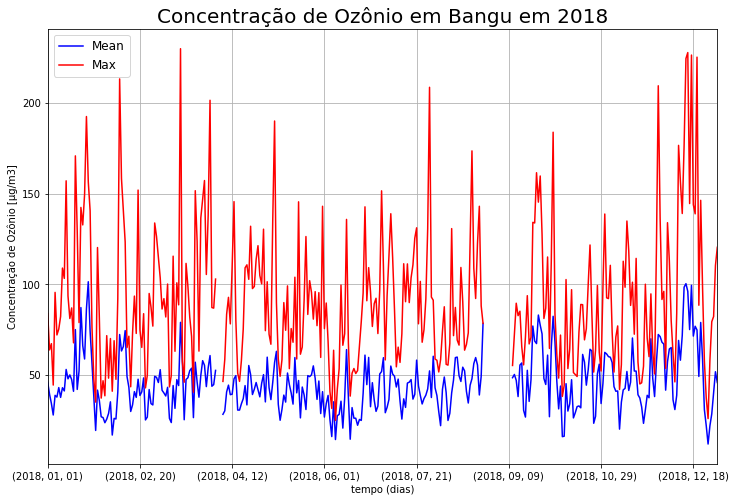
\includegraphics[width=\linewidth]{img/graphic4.png}
    \caption{Concentração de Ozônio em 2018.}
    \label{time-series}
\end{figure}

\subsection{Autocorrelação}

Precisamos encontrar padrões na série temporal, a fim de encontrar possíveis
tendências, não necessariamente lineares, sazonalidades ou mudanças cíclicas. Para
isso, utilizo uma medida de relação linear entre valores com atraso da série.
Definimos $r_k$ como essa medida entre os valores $y_t$ e $y_{t - k}$, para
todos os valores de $y_t$ capturados. Esse método é derivado da correlação de
Pearson. 

\begin{equation}
    \label{autocorrelation}
    r_k = \frac{\sum_{t = k + 1}^T (y_t - \overline{y})(y_{t - k} -
    \overline{y})}{\sum_{k=1}^T (y_t - \overline{y})^2}    
\end{equation}

A partir disso, é possível gerar a função de autocorrelação. Neste trabalho,
explorei essa função em relação aos meses e às horas. Em relação aos meses, meu
$k$ varia entre os valores de $0$ a $12$. De fato $r_0 = 1$. Espera-se que a
autocorrelação seja zero se o tempo não tenha influência sobre os dados. Nesse
caso, chamamos a série de ruído branco. Claro que como o conjunto de dados tem
tamanho finito, a autocorrelação dificilmente será $0$. Desta maneira, para
esses casos, é esperado que os valores estejam entre os limites $\pm
\frac{2}{\sqrt{T}}$ com probabilidade $95\%$, onde $T$ é o tamanho da amostra.
A figura \ref{acf-months} representa a função. Note o quão insignificantes se
tornam os limites. 

Valores altos para pequenos atrasos indicam tendência na série, já que
existe uma correlação alta entre os valores de um mês com os valores do mês
anterior. Entretanto, como o decréscimo não é suave, a tendência não é tão
observada. Também é interessante observar o efeito da sazonalidade em períodos
de 6 meses. Isso pode estar relacionado a período mais quente e frio, e a
alternância, nesses casos, da concentração de ozônio. 

No caso das horas, também foi observada alta correlação para valores de
atraso pequenos, mas o resultado foi pouco elucidativo. 

\begin{figure}  
    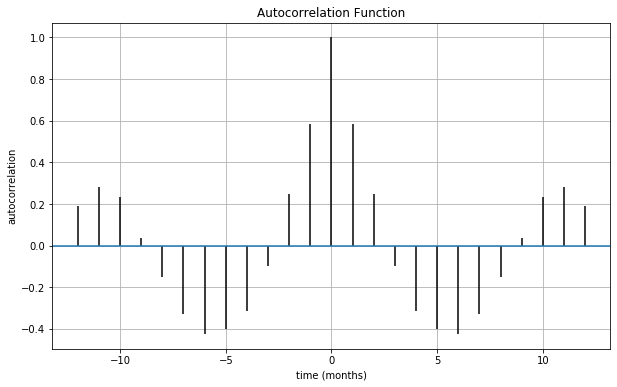
\includegraphics[width=\linewidth]{img/graphic3.png}
    \caption{Função de autocorrelação em relação aos meses. As linhas azuis
    representam os limites. }
    \label{acf-months}
\end{figure}

\subsection{Estacionariedade}

Uma série é dita estacionária quando ao passar do tempo, seus valores
mantem-se ao redor da média e variância constante. Quando uma série apresenta
tendência, ela não é estacionária. A importância de uma série estacionária é
para a realização do modelo, já que vários deles são descritos sobre séries
estacionárias. Para testar se nossa série temporal é estacionária,
consideremos o teste Dickey-Fuller Aumentado, um tipo de teste de uma raíz,
uma causa para a não estacionariedade.

$$H_0 : ~there~is~unit~root~(non~stationary)$$
$$H_1 : ~there~is~no~unit~root~(stationary)$$

Considero o nível de significância de 5\%. O p-valor do teste esteve na ordem
de $10^{-30}$, e a hipótese nula foi rejeitada. O teste foi realizado em
Python, através da função \textit{adfuller} do módulo para análide de séries
temporais \textit{statsmodels.tsa}. Para esse teste em Python, conferir
\cite{adf-test}. Outro fator importante de se analisar é a ergodicidade,
porém, nesse ensaio, assumirei a série como engórdica. 

\section{Modelando Séries Temporais}

Para modelar uma série temporal, a fim de fazer futuras predições, existem
diversos métodos apresentados pela literatura. Os dados consideram as máxima
média a cada 8h, que são consideradas para o cálculo do IQA no banco de dados.
Para os valores faltantes, preenchi com o valor anterior e deixo para futuros
trabalhos estudar métodos mais eficazes. Os dados não são afetados de forma
significativa por inflação, mudança na população ou calendário, pois o
intervalo temporal em anos não é muito grande. 

Para realizar os seguintes métodos, desenvolvo um processo para a análise do
resultado com o diagnóstico dos dos resíduos através do teste para
autocorrelação de \textit{Portmanteau}. Nesse teste, testamos se as primeiras $h$
autocorrelações são significantemente diferentes da esperada em ruído branco.
Existem várias estatísticas para esse teste, como, por exemplo, o teste
\textit{Box-Pierce} e, mais preciso, o teste \textit{Ljung-Box}, conforme
apêndice A. 

Para avaliar a precisão de nossas previsões, utilizo o método de
Cross-Validation para dividir os dados, mais de uma vez, em treino e teste. Ao
fim, para cada divisão temporal, calculo a precisão do modelo através do
método da Média Absoluta de Erros de Escala (Veja apêndice B) e, depois, faço
a média desse cálculo de previsão. 

\textbf{Métodos Estudados nesse trabalho: }
\begin{enumerate}
    \item Método da Média;
    \item Regressão Linear;
    \item Suavização Exponencial; 
\end{enumerate}

\subsection{Método da Média}

Nesse método de previsão, o modelo simplesmente afirma que a próxima
observação é a média das observações anteriores. Ele tem sua importância para
teste de sanidade e verificação dos métodos de análise de resultado.

\subsection{Regressão Linear}

A regressão linear admite que exista uma relação linear entre duas ou mais
séries temporais. Assim, 
$$y_t = \beta_0 + \beta_1x_{1,t} + ... + \beta_nx_{n,t}+ \epsilon_t$$
A variável $\epsilon$ captura tudo que as variáveis escolhidas não capturam.
Observe que os parâmetros indicam o quanto as variáveis são relacionadas e
como elas se relacionam (positivamente ou negativamente). Assumimos algumas
coisas sobre os erros: 

\begin{itemize}
    \item A média $0$;
    \item São não autocorrelacionados. Caso não fossem, existiria informação
    adicional que não foi extraída dos dados;
    \item São não relacionados com as variáveis preditoras, que representam as
    variáveis $x_{i,t}$. 
    \item É interessante, mas não necessário, que os erros sejam normalmente
    distribuídos. 
\end{itemize}

O método que utilizo para escolher os parâmetros é a estimação de mínimos
quadrados. Também, para esse modelo, lanço mão do coefieciente de
determinação, o $R^2$ (Veja Apêncice C).

As variáveis que utilizarei para esse modelo são Temperatura, Radiação Solar, 
Velocidade do Vento e Umidade Relativa. Essas quatro variáveis apresentam os
maiores valores absolutos de correlação e tem relação direta com a formação do
ozônio. A radiação solar, é um exemplo já construído na literatura e tem
relação direta com o ozônio \cite{solarRadiation}. 

Além disso, eu crio 11 variáveis indicadoras para os meses, a fim de capturar
a sazonalidade ou tendências em certos períodos. É importante dizer que não é 
necessária mais uma variável, pois ela estará incluída no parâmetro de
interceptação, que não acompanha variáveis independentes. Ao colocar essa
variável, podemos criar uma \textit{variável indicadora armadilha}. Essas
variáveis indicam $1$ para o mês correspondente e $0$ caso contrário. 

\subsection{Suavização Exponencial}

Proposta no final dos anos de 1950, por Brown, Holt e Winters, a suavização
exponenicial tem motivado diversos sucessos em previsões. Basicamente, esse
método faz uma média ponderada das observações passadas, só que esses pesos
decaem exponencialmente com o tempo. Especificamente, os pesos decrescem com
uma razão geométrica. Nesse método, existem diversas variações. Chamamos de
Suavização Exponencial Simples a seguinte equação:

$$\hat{y}_{T+1|T} = \sum_{j=0}^{T-1} \alpha(1 - \alpha)^jy_{T-j} + (1-
\alpha)l_0,$$
onde, os parâmetros $\alpha$ e $l_0$ devem ser estimados. $l_0$ a primeira
estimação, enquanto $\alpha$ é um valor entre $0$ e $1$ que indica o quando de
importância se dá aos eventos passados. 

Entretanto, nesse trabalho, desenvolvo um modelo para capturar a sazonalidade
dos dados, onde existe a equação de previsão e três equações de suavização: o
componente de tendência, o componente sazonal e o nível da suavização. Nesse
caso, existem mais dois parâmetros a serem estimados, além de um parâmetro de
sazonalidade que indica o número de períodos do ano. Esse modelo foi
desenvolvido por Holt e Winters. 

A fim de encontrar os parâmetros, também utilizo o método de minimização de
quadrados dos erros. 
    \section{Results}
\label{sec:results}

The results are separated by gas, but not by monitoring station. We present
more detailed results for only one (Tijuca station was chosen randomly), and after aggregated results
considering all the stations. This is done because we have more than
a hundred models to analyse. To deal with this diversity, the steps
(hyperparameters choice and evaluation) are automated. We are
making predictions one hour ahead and it is possible to compare with one day
ahead models. 

\subsection{Tijuca monitoring station}

The results follow the order specified in the above summary for each pollutant. 

\subsubsection{CO}

\subsubsection{O\texorpdfstring{$_3$}{3}}

{\em Simple linear regression}

\vspace{2mm}

Applying the simple linear regression, the $R^2$ in the testing set was 0.84,
what appears to be a good start fitting. The variable with greater t-statistic
was O$_3$ shifted by one hour. Other features with great t-statistic (more than
20) was, in
order, wind speedy, ozone lag 2, hour sin, UR, ozone lag 24, hour cos, and RS.
This is interesting because we have already observed the hourly seasonality
and by the formation of ozone, RS is expected to influence (not necessarily
linearly). The shifts were expected by the autocorrelation graph. Only some few features (3) had p-value greater that 0.05. The
F-statistic considering all variables was practically zero. One important
problem with this approach was the very big condition number (3.4e+06) given
the observed multicollinearity. Figure \ref{fig:histogram-residuals-slr} shows
the histogram of the residuals very similar to a normal distribution (as
assumed by the model).The kurtosis was nearly 3, while the skewness around
0.22. Jarque-Bera rejects the null hypotheses that skew and kurt are the same
as normal distribution, however.  The fitting result in testing data can be
partially observed in Figure \ref{fig:observed-fitting-ozone-tijuca}.

When the lags 1 and 2 are removed, that is, only using the lag 24, the metrics
get much worse. In special, $R^2$ is around 0.49.  

\begin{figure}
    \centering
    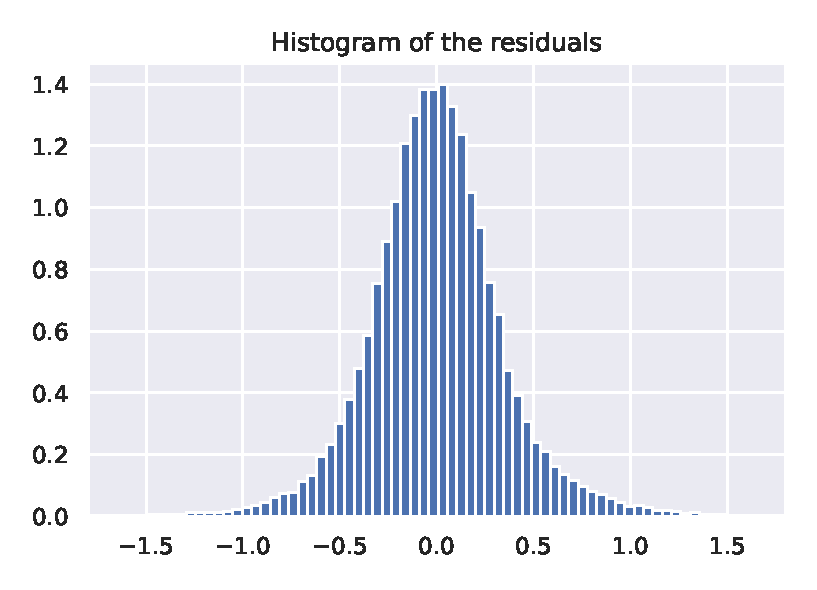
\includegraphics[width=0.45\textwidth]{histogram_residuals_slr.eps}
    \caption{Histogram of the residuals of simple linear regression model.}
    \label{fig:histogram-residuals-slr}
\end{figure}

\begin{figure*}
    \centering
    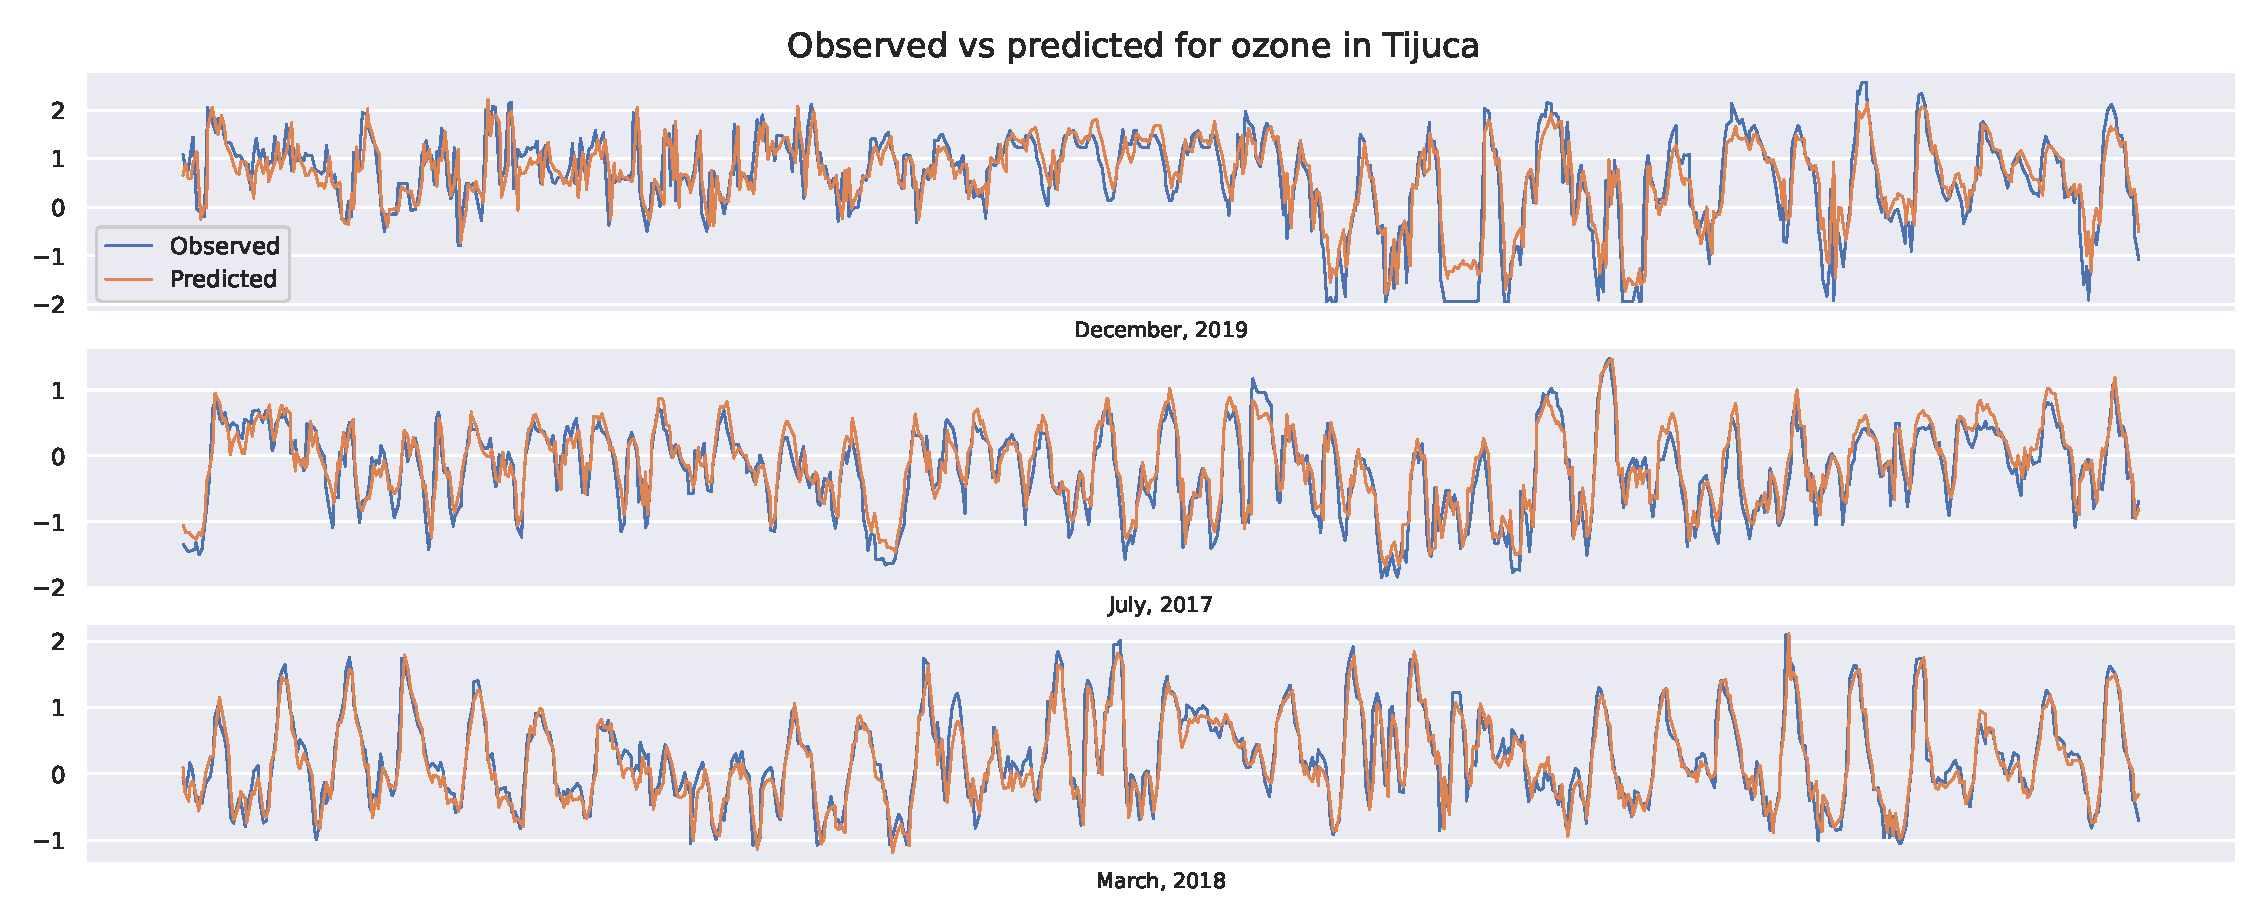
\includegraphics[width=\textwidth]{observed-fitting-ozone-tijuca.eps}
    \caption{Observed and predicted ozone values for different months in Tijuca.}
    \label{fig:observed-fitting-ozone-tijuca}
\end{figure*}

\subsubsection{PM\texorpdfstring{$_{10}$}{10}}

\subsubsection{AIQ}

\subsection{Aggregated results}

\subsubsection{CO}

\subsubsection{O\texorpdfstring{$_3$}{3}}

\subsubsection{PM\texorpdfstring{$_{10}$}{10}}

\subsubsection{AIQ}

\subsection{Model for other locations}

Here, we want to make predictions about pollutant levels at other not measured
sites. Given that each location has a specific model, the prediction
is the weighted mean regarding each prediction 



\begin{enumerate}
    \item 1 modelo para cada gás e cada estação. 
    \item Temos 7 opções de modelos até o momento (analisando friamente, 23 x
    7 = 161 modelos a serem fittados e analisados). 
    \item Como realizar tantos experimentos para cada modelo de forma
    automática? \com{A ideia é escrever um código para escolha de hiperparâmetros e
    reporte de resultados automaticamente.}
    \item Pegar uma estação para analisar os resultados mais cuidadosamente. 
    \item Testes de significância.  
\end{enumerate}

Lembrar de 

\begin{enumerate}
    \item Testar estacionaridade de cada série; 
    \item Lembrar de inverter os dados pelo power transformation: ler p2, fazer power transform. 
\end{enumerate}



\section{Discussion and Future work}
\label{sec:discussion}


\section{Conclusion}
\label{sec:conclusion}

    }
\else 
    {
    \section{Introduction}

\lettrine[findent=2pt]{\textbf{R}}{}io de Janeiro city (Brazil) is one of the
most beautiful cities in the world, according to the travel website Conde Nast
Traveler \cite{travelRio}. This thought is shared among tourists and
residents.

\begin{enumerate}
    \item What is the problem? 
    \item Why is it important? 
    \item What is your basic approach? 
    \item A short discussion of how it fits into related work in the area is also desirable.
    \item Basic results. 
    \item Conclusions
\end{enumerate}

\section{Problem definition}

\begin{enumerate}
    \item What is the problem?
    \item What are the inputs and outputs mathematically. 
\end{enumerate}
    \section{Background of air pollution}

Air pollution is a mixture of particles and gases, often not visible to human
eyes. The visible forms are widely known, such as smoke, soot and mold.
\com{The quality air index, calculated based on the levels of the gases, is
available in a diary report}, as presented in image XXX.  

\subsection{Polluting gases}

The atmosphere of the Earth is a dynamic and complex system of natural gases,
which are necessary to life, according to \cite{gases}. The planet has a
defense mechanism that absorbs part of these fases, what forms a cycle.
However, high levels of gases concentration can cause several effects in the
living beings. The polluting gases include: 

\begin{itemize}
    \item \textbf{Óxidos de Carbono:} O monóxido de carbono (CO) é oriundo da
    combustão incompleta e não apresenta cheiro ou cor. Já o dióxido de
    carbono é um gás que contribui para o efeito estufa e, em excesso na
    atmosfera, devido à queima de combustíveis fósseis, pode causas sérios
    danos.  
    \item \textbf{Óxidos de Nitrogênio:} Também emitidos por veículos e
    tem uma aparência marrom. O dióxido de nitrogênio é um dos gases mais
    perigosos para a poluição do ar, e sua toxidade é facilmente
    identificável. 
    \item \textbf{Óxidos de Enxofre:} Causa primária da chuva ácida, muito
    comum na Europa. É natural após erupções vulcânicas. É uma forte causa de
    problemas respiratórios. 
    \item \textbf{Ozônio:} O gás ozônio ($O_3$) contém três átomos de oxigênio. Até pequenas
    concentrações desse gás são consideradas tóxicas e explosivas. Ele ocorre
    naturalmente na atmosfera, porém em pequenas quantidades, quando absorve
    radiação ultravioleta. Em condições especiais, óxidos de nitrogênio e
    hidrocarbonos podem produzir ozônio em concentração alta o suficiente para
    causar irritação nos olhos e na mucosa. 
\end{itemize}



    \section{Methodology}
\label{sec:methodology}

\BL{E}xploratory data analysis is the first step into the project, after
identifying the problem. The proposed EDA includes visualization and descriptive statistics to
summarize the most relevant information to have insights. After this, we make
data preprocessing, which includes missing data imputation, outlies, and
feature engineering.   

The evaluation methods for the algorithms are the mean absolute error (MAE), the root
mean squared error (RMSE), and the normalized RMSE (nRMSE). The methods were
trained using 70\% of the available data, considering the first years. The
software used for performing this experimental phase was developed in Python (version 3.9), mainly using the Pandas and Scikit-learn.

    \section{Exploratory data analysis}

\subsection{Data description}

The dataset used in this study was extracted from the project MonitorAr
\cite{dataset-rio-ar-quality}. The table contains hourly data observations, separated by
pollutant, weather condition, and monitoring stations' characteristics from
the city of Rio de Janeiro. Table
\ref{tab:measured-data} informs the most important variables used, and Table
\ref{tab:pollutants-measured} indicates the measured pollutants. The events were collected between January 1,
2011,
and March 31, 2021. A total of 661,662 records were used. 

\begin{table*}[t]
    \centering
    \begin{tabular}{c|c|c|c|}
        \cline{2-4}
                                                                                 & \textbf{Name} & \textbf{Type} & \textbf{Description}              \\ \hline
        \multicolumn{1}{|c|}{\multirow{7}{*}{\textbf{Meterological conditions}}} & Chuva         & float         & Rainfall (mm)                     \\ \cline{2-4} 
        \multicolumn{1}{|c|}{}                                                   & Pres          & float         & Atmospheric Pressure (mbar)       \\ \cline{2-4} 
        \multicolumn{1}{|c|}{}                                                   & RS            & float         & Solar radiation (w/m2)            \\ \cline{2-4} 
        \multicolumn{1}{|c|}{}                                                   & Temp          & float         & Temperature (°C)                  \\ \cline{2-4} 
        \multicolumn{1}{|c|}{}                                                   & UR            & float         & Relative humidity (\%)            \\ \cline{2-4} 
        \multicolumn{1}{|c|}{}                                                   & Dir\_Vento    & float         & Wind direction (°)                \\ \cline{2-4} 
        \multicolumn{1}{|c|}{}                                                   & Vel\_Vento    & float         & Wind speed (m/s)                  \\ \hline
        \multicolumn{1}{|c|}{\multirow{5}{*}{\textbf{Measurement conditions}}}   & Data          & datetime      & Measurement date and hour         \\ \cline{2-4} 
        \multicolumn{1}{|c|}{}                                                   & CodNum        & ineger        & Number of the monitoring station  \\ \cline{2-4} 
        \multicolumn{1}{|c|}{}                                                   & Estação       & string        & Name of the monitoring station    \\ \cline{2-4} 
        \multicolumn{1}{|c|}{}                                                   & Lat           & float         & Latitude position of the station  \\ \cline{2-4} 
        \multicolumn{1}{|c|}{}                                                   & Lon           & float         & Longitude position of the station \\ \hline
        \end{tabular}
    \caption{Measured parameters by the program MonitorAr.}
    \label{tab:measured-data}
\end{table*}

\begin{table*}[b]
    \centering
    \begin{tabular}{|c|c|}
    \hline
    \textbf{Monitoring station}        & \textbf{Measured gases/particulates}              \\ \hline
    Centro (CA)             & O$_3$, CO, PM$_{10}$                              \\ \hline
    Copacabana (AV)         & SO$_2$, O$_3$, CO, PM$_{10}$                      \\ \hline
    São Cristóvão (SC)      & SO$_2$, O$_3$, CO, PM$_{10}$                      \\ \hline
    Tijuca (SP)             & SO$_2$, NOx, O$_3$, CO, PM$_{10}$                 \\ \hline
    Irajá (IR)              & SO$_2$, NOx, O$_3$, CO, HC, PM$_{2.5}$, PM$_{10}$ \\ \hline
    Bangu (BG)              & SO$_2$, NOx, O$_3$, CO, HC, PM$_{10}$             \\ \hline
    Campo Grande (CG)       & SO$_2$, NOx, O$_3$, CO, HC, PM$_{10}$             \\ \hline
    Pedra de Guaratiba (PG) & O$_3$, PM$_{10}$                                  \\ \hline
    \end{tabular}
    \caption{Pollutant data measured by each monitoring station. CO and HC are measured in (ppm), while the others are measured in (µg/m3).}
    \label{tab:pollutants-measured}
\end{table*}

\begin{enumerate}
    \item Reportar valores nulos da chuva e índice de missing values
\end{enumerate}

\begin{enumerate}
    \item Gráficos dos gases e interpretação de alguns deles. Analisar curtose
    e assimetria.
    \item Mensurações temporais de alguns gases. Selecionar alguns poucos
    \item Testes de estacionariedade nas séries utilizadas. 
    \item Mais alguns gráficos de visualização. 
\end{enumerate}

\subsection{Data preprocessing}

The data preprocessing is an important step before the usage of machine
learning algorithms, in order to report robust and neat results. 

\begin{enumerate}
    \item Imputation of missing data
    \item Handling outliers
    \item normalization and standardization. 
    \item feature engineering
\end{enumerate}

\subsubsection{Missing data imputation}

In this dataset, there is two types of missing data: (1) monitoring stations
do not measure all pollutants by construction. For instance, it is not
measured NOx in Centro and Copacabana; and (2) monitoring stations did not
measure in a period for some reason. We have to deal with them in two
different ways. 

\begin{enumerate}
    \item Possíveis formas de imputação: estimação polinomial de 2ª ordem.
    Alguns testes simples pode ser interessante. Para locais onde não há
    estimação, não faz sentido imputar. 
\end{enumerate}

\subsubsection{Data transformation}

\begin{enumerate}
    \item Transformação Yeo-Johnson 
\end{enumerate}

\subsubsection{Feature extraction}

From the variable {\tt Data}, we can observe (Figure
\ref{fig:histogram-obs-years}) that 2011 has less observations, because there
were only four of the eight stations operating. For that reason, we do not
consider the data from this year. 

\begin{figure}
    \begin{center}
        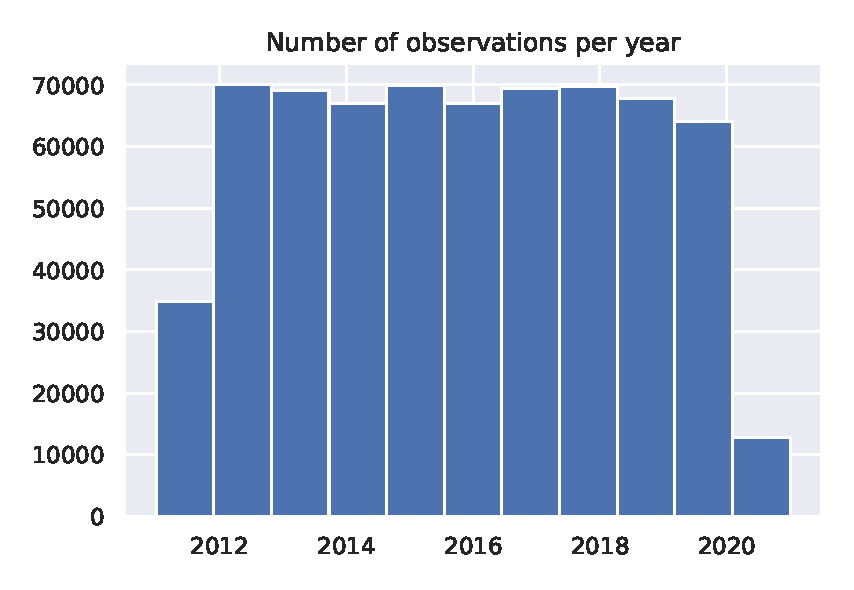
\includegraphics[width=0.47\textwidth]{histogram.eps}
    \end{center}
    \caption{Number of hourly measurements per year. In 2011, only half of the monitoring stations worked.}
    \label{fig:histogram-obs-years}
\end{figure}

\begin{enumerate}
    \item Analisar sazonalidade. Adicionar termo seno e cosseno de forma que
    exista sazonalidade diária, isto é, 
    $$
    \text{hour\_sin} = \sin(2\pi \text{ hour}/24)
    $$
    \item Create variable season.   
\end{enumerate}
    \section{Results}
\label{sec:results}

The results are separated by gas, but not by monitoring station. We present
more detailed results for only one (Tijuca station was chosen randomly), and after aggregated results
considering all the stations. This is done because we have more than
a hundred models to analyse. To deal with this diversity, the steps
(hyperparameters choice and evaluation) are automated. We are
making predictions one hour ahead and it is possible to compare with one day
ahead models. 

\subsection{Tijuca monitoring station}

The results follow the order specified in the above summary for each pollutant. 

\subsubsection{CO}

\subsubsection{O\texorpdfstring{$_3$}{3}}

{\em Simple linear regression}

\vspace{2mm}

Applying the simple linear regression, the $R^2$ in the testing set was 0.84,
what appears to be a good start fitting. The variable with greater t-statistic
was O$_3$ shifted by one hour. Other features with great t-statistic (more than
20) was, in
order, wind speedy, ozone lag 2, hour sin, UR, ozone lag 24, hour cos, and RS.
This is interesting because we have already observed the hourly seasonality
and by the formation of ozone, RS is expected to influence (not necessarily
linearly). The shifts were expected by the autocorrelation graph. Only some few features (3) had p-value greater that 0.05. The
F-statistic considering all variables was practically zero. One important
problem with this approach was the very big condition number (3.4e+06) given
the observed multicollinearity. Figure \ref{fig:histogram-residuals-slr} shows
the histogram of the residuals very similar to a normal distribution (as
assumed by the model).The kurtosis was nearly 3, while the skewness around
0.22. Jarque-Bera rejects the null hypotheses that skew and kurt are the same
as normal distribution, however.  The fitting result in testing data can be
partially observed in Figure \ref{fig:observed-fitting-ozone-tijuca}.

When the lags 1 and 2 are removed, that is, only using the lag 24, the metrics
get much worse. In special, $R^2$ is around 0.49.  

\begin{figure}
    \centering
    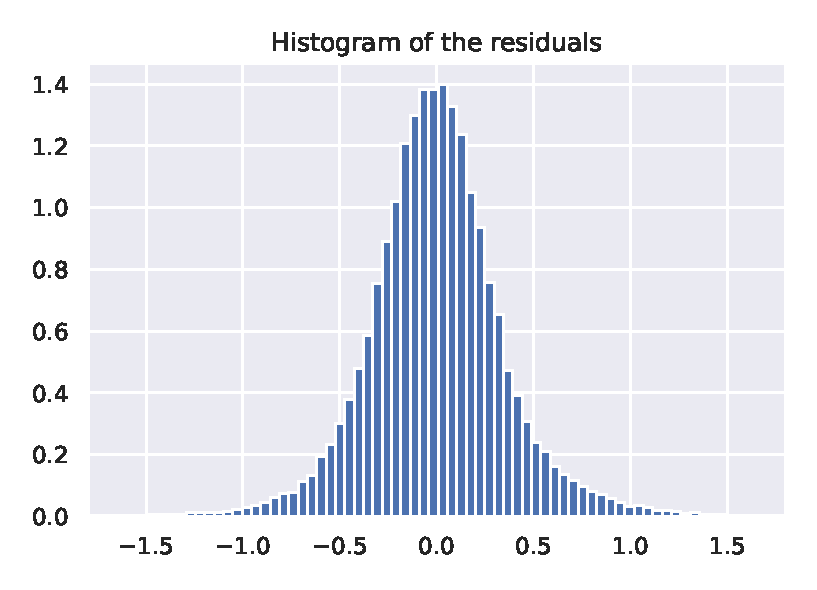
\includegraphics[width=0.45\textwidth]{histogram_residuals_slr.eps}
    \caption{Histogram of the residuals of simple linear regression model.}
    \label{fig:histogram-residuals-slr}
\end{figure}

\begin{figure*}
    \centering
    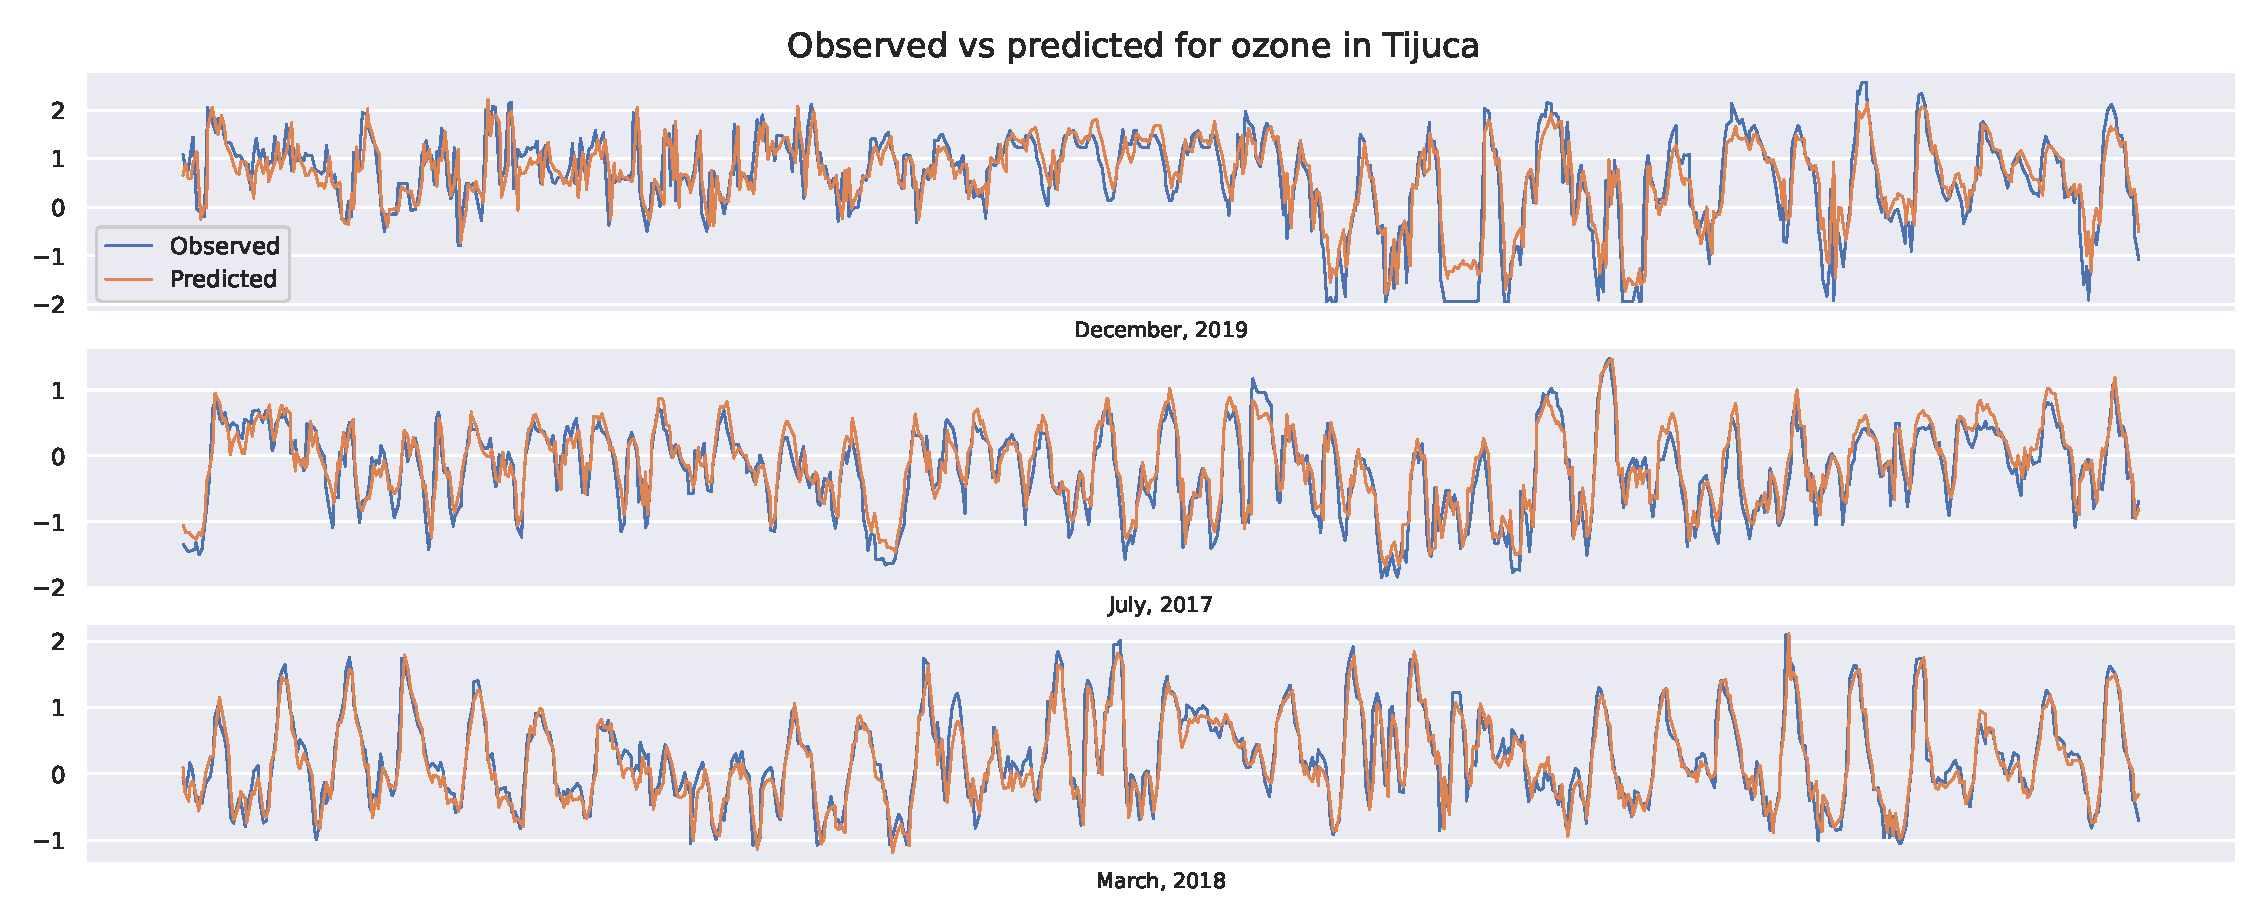
\includegraphics[width=\textwidth]{observed-fitting-ozone-tijuca.eps}
    \caption{Observed and predicted ozone values for different months in Tijuca.}
    \label{fig:observed-fitting-ozone-tijuca}
\end{figure*}

\subsubsection{PM\texorpdfstring{$_{10}$}{10}}

\subsubsection{AIQ}

\subsection{Aggregated results}

\subsubsection{CO}

\subsubsection{O\texorpdfstring{$_3$}{3}}

\subsubsection{PM\texorpdfstring{$_{10}$}{10}}

\subsubsection{AIQ}

\subsection{Model for other locations}

Here, we want to make predictions about pollutant levels at other not measured
sites. Given that each location has a specific model, the prediction
is the weighted mean regarding each prediction 



\begin{enumerate}
    \item 1 modelo para cada gás e cada estação. 
    \item Temos 7 opções de modelos até o momento (analisando friamente, 23 x
    7 = 161 modelos a serem fittados e analisados). 
    \item Como realizar tantos experimentos para cada modelo de forma
    automática? \com{A ideia é escrever um código para escolha de hiperparâmetros e
    reporte de resultados automaticamente.}
    \item Pegar uma estação para analisar os resultados mais cuidadosamente. 
    \item Testes de significância.  
\end{enumerate}

Lembrar de 

\begin{enumerate}
    \item Testar estacionaridade de cada série; 
    \item Lembrar de inverter os dados pelo power transformation: ler p2, fazer power transform. 
\end{enumerate}



\section{Discussion and Future work}
\label{sec:discussion}


\section{Conclusion}
\label{sec:conclusion}

    }
\fi

    \newpage

    %\appendix

    %\newpage

\twocolumn[
    \begin{@twocolumnfalse}
        \bibliography{sections/biblio} 
    \end{@twocolumnfalse}
]

\end{document}